\clearpage
\SourceLeaf{257}%
\begin{center}
{\Large\textsc{Theorem aus der Sph\"arologie.}}
\end{center}

\begin{center}\begin{minipage}{\linewidth}\centering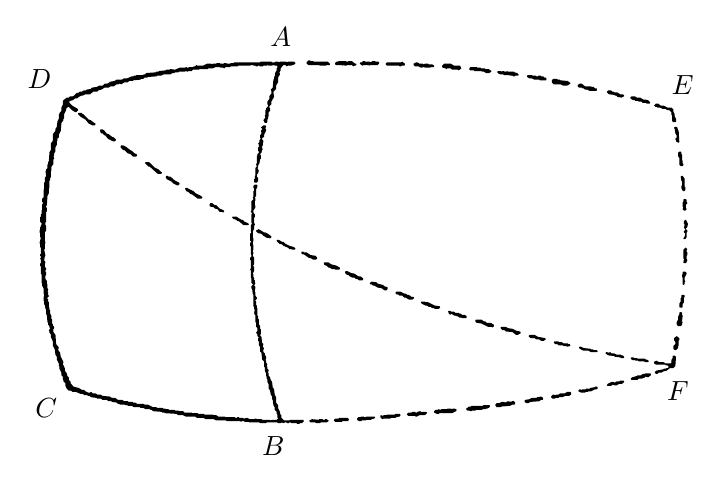
\begin{tikzpicture}[x=0.00843486cm,y=-0.00843486cm]
\fill[even odd rule] (458,625) -- (458,626) -- (460,628) -- (467,628) -- (468,629) -- (474,629) -- (475,628) -- (484,628) -- (487,626) -- (487,625) -- (484,623) -- (482,623) -- (481,624) -- (479,624) -- (478,623) -- (473,623) -- (472,624) -- (462,623) -- cycle
(495,625) -- (497,627) -- (507,627) -- (508,626) -- (516,626) -- (518,624) -- (516,621) -- (503,621) -- (502,622) -- (498,622) -- (496,623) -- cycle
(530,624) -- (533,626) -- (536,626) -- (537,625) -- (543,625) -- (544,624) -- (551,624) -- (552,623) -- (556,622) -- (557,620) -- (556,619) -- (544,619) -- (543,620) -- (541,620) -- (540,619) -- (536,619) -- (535,620) -- (532,620) -- (530,622) -- cycle
(595,616) -- (594,615) -- (588,615) -- (587,616) -- (575,616) -- (574,617) -- (570,617) -- (569,618) -- (566,617) -- (565,618) -- (565,620) -- (568,623) -- (570,622) -- (580,622) -- (581,621) -- (588,621) -- (589,620) -- (594,619) -- (595,618) -- cycle
(635,613) -- (634,612) -- (626,612) -- (625,611) -- (621,612) -- (620,613) -- (618,613) -- (617,612) -- (613,612) -- (612,613) -- (608,613) -- (606,614) -- (605,616) -- (607,618) -- (617,618) -- (618,619) -- (620,619) -- (624,617) -- (631,617) -- (633,616) -- (635,614) -- cycle
(680,609) -- (677,607) -- (674,607) -- (673,608) -- (671,607) -- (666,607) -- (665,608) -- (657,608) -- (656,609) -- (652,608) -- (651,609) -- (648,609) -- (646,611) -- (646,613) -- (650,615) -- (653,615) -- (654,614) -- (673,614) -- (679,611) -- cycle
(730,603) -- (729,602) -- (720,602) -- (719,603) -- (702,603) -- (701,604) -- (698,604) -- (696,606) -- (695,606) -- (694,608) -- (696,610) -- (699,610) -- (700,611) -- (702,611) -- (703,610) -- (708,610) -- (709,609) -- (718,609) -- (719,608) -- (723,608) -- (724,607) -- (726,607) -- (728,606) -- (730,604) -- cycle
(768,598) -- (766,596) -- (763,596) -- (762,597) -- (757,596) -- (753,598) -- (751,597) -- (748,597) -- (744,599) -- (740,599) -- (738,601) -- (738,602) -- (740,605) -- (746,605) -- (747,604) -- (760,603) -- (764,601) -- (767,601) -- (768,600) -- cycle
(810,591) -- (807,589) -- (801,590) -- (800,591) -- (793,591) -- (789,593) -- (783,594) -- (782,595) -- (782,597) -- (785,599) -- (787,599) -- (791,597) -- (804,596) -- (807,594) -- (809,594) -- (810,593) -- cycle
(852,583) -- (851,582) -- (846,582) -- (843,584) -- (836,584) -- (833,586) -- (830,586) -- (829,587) -- (825,586) -- (822,589) -- (822,590) -- (824,592) -- (828,592) -- (829,591) -- (833,591) -- (834,590) -- (839,590) -- (843,588) -- (849,588) -- (852,586) -- cycle
(892,575) -- (891,574) -- (888,574) -- (887,575) -- (881,576) -- (880,577) -- (875,577) -- (874,578) -- (869,578) -- (868,579) -- (865,578) -- (863,580) -- (863,581) -- (867,583) -- (873,583) -- (874,582) -- (877,582) -- (878,581) -- (882,581) -- (888,578) -- (891,578) -- (892,577) -- cycle
(932,566) -- (931,565) -- (926,565) -- (925,566) -- (921,566) -- (918,568) -- (916,567) -- (913,567) -- (907,570) -- (906,572) -- (907,573) -- (912,573) -- (915,571) -- (917,572) -- (921,572) -- (924,570) -- (928,570) -- (930,569) -- (932,567) -- cycle
(972,555) -- (971,554) -- (964,554) -- (963,555) -- (960,555) -- (957,557) -- (952,557) -- (951,558) -- (944,560) -- (942,562) -- (942,563) -- (943,564) -- (952,564) -- (954,562) -- (959,562) -- (960,561) -- (962,561) -- (964,559) -- (968,560) -- (972,557) -- cycle
(942,531) -- (942,532) -- (944,534) -- (948,534) -- (949,535) -- (953,535) -- (954,536) -- (962,536) -- (963,537) -- (968,537) -- (969,536) -- (968,534) -- (964,533) -- (963,532) -- (952,532) -- (951,531) -- (947,531) -- (946,530) -- (943,530) -- cycle
(1010,529) -- (1007,527) -- (1005,528) -- (1005,531) -- (1003,534) -- (1003,538) -- (1002,539) -- (994,539) -- (991,537) -- (984,537) -- (981,535) -- (978,536) -- (977,537) -- (977,539) -- (980,541) -- (994,541) -- (995,542) -- (997,542) -- (999,544) -- (998,546) -- (996,546) -- (995,547) -- (992,547) -- (991,548) -- (980,550) -- (978,552) -- (978,553) -- (980,555) -- (982,555) -- (984,553) -- (988,553) -- (991,551) -- (996,550) -- (1001,546) -- (1006,546) -- (1009,543) -- cycle
(904,523) -- (904,524) -- (908,527) -- (917,528) -- (918,529) -- (926,530) -- (927,531) -- (931,531) -- (932,530) -- (932,529) -- (930,527) -- (928,527) -- (927,526) -- (921,526) -- (917,524) -- (913,524) -- (911,522) -- (909,523) -- (905,522) -- cycle
(864,515) -- (865,517) -- (871,520) -- (878,520) -- (882,522) -- (891,522) -- (892,521) -- (891,519) -- (886,519) -- (885,518) -- (882,518) -- (881,517) -- (871,516) -- (867,514) -- (865,514) -- cycle
(826,507) -- (826,508) -- (828,510) -- (831,510) -- (834,512) -- (840,512) -- (841,513) -- (845,513) -- (846,514) -- (850,513) -- (851,512) -- (850,510) -- (848,510) -- (847,509) -- (841,509) -- (838,507) -- (834,507) -- (833,506) -- (827,506) -- cycle
(1011,498) -- (1007,501) -- (1007,504) -- (1009,507) -- (1009,510) -- (1006,513) -- (1006,517) -- (1008,519) -- (1010,519) -- (1013,516) -- (1013,513) -- (1014,512) -- (1014,505) -- (1015,504) -- (1015,501) -- cycle
(788,498) -- (791,501) -- (797,501) -- (800,503) -- (804,503) -- (807,505) -- (811,505) -- (814,503) -- (813,501) -- (802,499) -- (797,496) -- (790,496) -- cycle
(746,485) -- (746,486) -- (749,489) -- (752,489) -- (754,491) -- (764,492) -- (769,496) -- (772,496) -- (776,494) -- (776,492) -- (775,491) -- (770,490) -- (764,487) -- (757,486) -- (754,484) -- (747,484) -- cycle
(708,474) -- (708,476) -- (710,478) -- (717,479) -- (727,484) -- (732,484) -- (734,485) -- (736,483) -- (736,481) -- (731,478) -- (725,478) -- (723,476) -- (721,476) -- (717,473) -- (709,473) -- cycle
(1018,462) -- (1016,462) -- (1015,463) -- (1015,465) -- (1013,469) -- (1013,473) -- (1011,477) -- (1011,480) -- (1013,483) -- (1017,483) -- (1019,481) -- (1019,479) -- (1020,478) -- (1019,476) -- (1020,467) -- (1019,466) -- (1019,463) -- cycle
(667,461) -- (668,464) -- (670,466) -- (671,465) -- (673,465) -- (676,467) -- (678,467) -- (679,468) -- (681,468) -- (684,470) -- (687,470) -- (688,471) -- (694,471) -- (695,470) -- (695,468) -- (692,466) -- (688,466) -- (686,464) -- (684,464) -- (683,463) -- (678,463) -- (675,461) -- (671,461) -- (670,460) -- (668,460) -- cycle
(626,447) -- (627,449) -- (633,452) -- (635,452) -- (638,454) -- (641,454) -- (643,456) -- (646,456) -- (647,457) -- (653,457) -- (655,455) -- (654,453) -- (647,452) -- (637,447) -- (633,447) -- (632,446) -- (627,446) -- cycle
(1022,436) -- (1019,436) -- (1018,437) -- (1018,440) -- (1017,441) -- (1017,446) -- (1015,449) -- (1015,454) -- (1016,455) -- (1019,455) -- (1020,454) -- (1020,450) -- (1022,447) -- (1022,440) -- (1023,439) -- (1023,437) -- cycle
(588,432) -- (588,434) -- (589,435) -- (591,435) -- (594,437) -- (598,437) -- (601,440) -- (603,440) -- (608,443) -- (613,443) -- (616,441) -- (615,439) -- (612,439) -- (608,436) -- (606,436) -- (603,434) -- (601,434) -- (595,431) -- (589,431) -- cycle
(549,418) -- (550,420) -- (552,420) -- (554,422) -- (556,422) -- (561,425) -- (567,426) -- (571,429) -- (574,429) -- (576,427) -- (576,425) -- (575,424) -- (571,423) -- (569,421) -- (561,419) -- (559,417) -- (552,416) -- cycle
(1024,401) -- (1021,401) -- (1020,402) -- (1020,405) -- (1019,406) -- (1019,409) -- (1020,410) -- (1020,420) -- (1021,421) -- (1023,420) -- (1023,417) -- (1024,416) -- (1023,414) -- (1023,410) -- (1026,404) -- (1026,403) -- cycle
(512,401) -- (512,403) -- (515,406) -- (517,406) -- (519,408) -- (523,410) -- (526,410) -- (528,412) -- (530,412) -- (533,414) -- (538,414) -- (539,413) -- (539,411) -- (535,408) -- (532,408) -- (526,404) -- (521,403) -- (515,400) -- (513,400) -- cycle
(480,388) -- (480,390) -- (481,391) -- (484,392) -- (487,395) -- (489,395) -- (492,397) -- (496,397) -- (497,398) -- (503,398) -- (504,397) -- (504,395) -- (499,392) -- (491,390) -- (487,387) -- (481,387) -- cycle
(446,372) -- (446,373) -- (448,375) -- (450,375) -- (457,380) -- (461,381) -- (464,383) -- (468,383) -- (470,381) -- (470,380) -- (467,377) -- (460,376) -- (454,372) -- (450,372) -- (449,371) -- (447,371) -- cycle
(1025,365) -- (1024,365) -- (1021,368) -- (1021,381) -- (1022,382) -- (1021,387) -- (1022,388) -- (1025,388) -- (1027,384) -- (1026,382) -- (1026,377) -- (1027,376) -- (1027,372) -- (1026,371) -- (1026,369) -- (1027,367) -- cycle
(409,354) -- (409,355) -- (413,359) -- (417,360) -- (419,362) -- (426,365) -- (428,367) -- (431,367) -- (432,368) -- (436,368) -- (437,367) -- (437,366) -- (435,364) -- (428,362) -- (422,359) -- (419,356) -- (417,356) -- (412,353) -- (410,353) -- cycle
(378,339) -- (378,340) -- (381,343) -- (386,344) -- (389,347) -- (394,350) -- (397,350) -- (399,351) -- (401,349) -- (401,348) -- (396,344) -- (392,342) -- (390,342) -- (382,337) -- cycle
(1025,323) -- (1024,323) -- (1022,325) -- (1022,329) -- (1023,330) -- (1022,335) -- (1024,337) -- (1024,338) -- (1022,340) -- (1022,342) -- (1024,344) -- (1023,348) -- (1021,351) -- (1022,352) -- (1024,352) -- (1026,349) -- (1026,342) -- (1027,341) -- (1027,339) -- (1025,337) -- (1025,336) -- (1027,334) -- (1028,329) -- cycle
(342,319) -- (343,321) -- (348,323) -- (350,325) -- (352,325) -- (359,331) -- (366,331) -- (367,330) -- (366,328) -- (361,326) -- (358,323) -- (356,323) -- (348,318) -- (343,318) -- cycle
(308,299) -- (308,302) -- (309,303) -- (314,304) -- (316,306) -- (320,307) -- (323,311) -- (327,311) -- (328,312) -- (330,311) -- (330,310) -- (328,308) -- (323,306) -- (318,301) -- (316,301) -- (312,298) -- (309,298) -- cycle
(1022,292) -- (1021,293) -- (1021,296) -- (1020,297) -- (1020,303) -- (1021,304) -- (1020,307) -- (1022,309) -- (1024,309) -- (1026,307) -- (1025,305) -- (1025,300) -- (1027,298) -- (1027,297) -- (1026,296) -- (1026,293) -- (1025,292) -- cycle
(271,276) -- (273,280) -- (276,281) -- (279,284) -- (282,285) -- (290,291) -- (296,291) -- (297,290) -- (297,289) -- (295,287) -- (287,283) -- (284,280) -- (274,275) -- (272,275) -- cycle
(1018,257) -- (1017,258) -- (1018,264) -- (1019,265) -- (1019,271) -- (1018,272) -- (1018,275) -- (1020,279) -- (1022,280) -- (1024,278) -- (1024,274) -- (1023,273) -- (1023,261) -- (1020,257) -- cycle
(242,258) -- (242,260) -- (244,262) -- (250,265) -- (253,268) -- (259,271) -- (261,271) -- (263,269) -- (262,267) -- (256,264) -- (249,258) -- (246,258) -- (245,257) -- (243,257) -- cycle
(211,237) -- (211,238) -- (216,243) -- (218,243) -- (229,253) -- (231,254) -- (234,254) -- (236,253) -- (236,251) -- (235,251) -- (231,247) -- (225,244) -- (218,237) -- (216,236) -- (212,236) -- cycle
(1016,220) -- (1013,222) -- (1013,227) -- (1015,230) -- (1015,240) -- (1017,242) -- (1020,242) -- (1021,241) -- (1021,239) -- (1020,238) -- (1020,234) -- (1019,233) -- (1019,225) -- (1018,224) -- (1018,221) -- cycle
(174,212) -- (174,214) -- (178,218) -- (180,218) -- (185,223) -- (189,224) -- (193,228) -- (197,228) -- (199,226) -- (198,224) -- (195,223) -- (191,219) -- (190,219) -- (182,213) -- (178,211) -- (175,211) -- cycle
(143,188) -- (144,192) -- (145,193) -- (147,193) -- (150,196) -- (151,196) -- (155,201) -- (163,205) -- (165,205) -- (167,203) -- (167,202) -- (164,199) -- (161,198) -- (156,194) -- (153,193) -- (149,188) -- (147,187) -- (144,187) -- cycle
(1008,183) -- (1007,185) -- (1008,186) -- (1009,193) -- (1011,196) -- (1011,199) -- (1009,201) -- (1009,202) -- (1010,203) -- (1010,205) -- (1014,207) -- (1015,206) -- (1014,189) -- (1013,188) -- (1012,184) -- (1011,183) -- cycle
(392,181) -- (389,181) -- (385,184) -- (387,186) -- (387,187) -- (385,189) -- (386,191) -- (386,193) -- (384,196) -- (384,199) -- (385,201) -- (383,203) -- (383,206) -- (381,208) -- (382,210) -- (382,213) -- (381,214) -- (381,219) -- (382,220) -- (382,222) -- (380,224) -- (380,226) -- (379,227) -- (379,238) -- (378,239) -- (379,243) -- (377,245) -- (377,256) -- (376,257) -- (376,261) -- (375,262) -- (375,266) -- (376,267) -- (379,267) -- (381,265) -- (381,260) -- (379,258) -- (379,255) -- (381,253) -- (382,249) -- (380,245) -- (381,244) -- (381,241) -- (383,238) -- (384,232) -- (385,231) -- (385,226) -- (384,224) -- (386,222) -- (387,218) -- (388,217) -- (387,215) -- (387,212) -- (388,211) -- (388,207) -- (389,206) -- (389,204) -- (387,202) -- (387,200) -- (390,198) -- (390,195) -- (393,189) -- (393,187) -- (392,186) -- (393,182) -- cycle
(110,162) -- (110,164) -- (114,168) -- (121,172) -- (126,178) -- (132,181) -- (135,181) -- (136,180) -- (136,178) -- (135,177) -- (134,177) -- (129,173) -- (126,172) -- (118,164) -- (117,164) -- (115,162) -- cycle
(977,151) -- (979,153) -- (981,153) -- (982,154) -- (986,154) -- (990,156) -- (994,156) -- (997,158) -- (1000,158) -- (1003,161) -- (1003,165) -- (1004,166) -- (1004,174) -- (1006,176) -- (1009,176) -- (1010,175) -- (1010,171) -- (1008,167) -- (1008,164) -- (1006,160) -- (1006,157) -- (1003,154) -- (997,154) -- (991,151) -- (987,151) -- (983,148) -- (980,148) -- cycle
(941,139) -- (942,141) -- (946,143) -- (948,143) -- (949,144) -- (953,144) -- (954,145) -- (958,145) -- (960,147) -- (965,147) -- (966,148) -- (970,148) -- (971,147) -- (971,146) -- (968,143) -- (966,143) -- (965,142) -- (961,142) -- (956,139) -- (951,139) -- (948,137) -- (943,137) -- cycle
(906,130) -- (906,131) -- (909,134) -- (917,135) -- (918,136) -- (920,136) -- (922,138) -- (928,139) -- (932,137) -- (932,136) -- (930,134) -- (926,134) -- (921,131) -- (917,131) -- (916,130) -- (914,130) -- (912,128) -- (908,128) -- cycle
(862,120) -- (862,122) -- (864,124) -- (868,124) -- (869,125) -- (871,125) -- (873,127) -- (876,127) -- (880,129) -- (890,129) -- (891,128) -- (891,126) -- (890,125) -- (888,125) -- (886,123) -- (883,123) -- (882,122) -- (873,122) -- (868,118) -- (865,118) -- cycle
(823,113) -- (823,116) -- (826,119) -- (836,119) -- (840,121) -- (846,121) -- (851,118) -- (851,117) -- (847,114) -- (836,113) -- (835,112) -- (832,112) -- (831,111) -- (825,111) -- cycle
(786,106) -- (786,108) -- (789,110) -- (793,110) -- (797,112) -- (804,112) -- (805,113) -- (814,113) -- (815,112) -- (815,110) -- (814,109) -- (812,109) -- (810,107) -- (807,107) -- (806,106) -- (803,106) -- (802,107) -- (800,107) -- (799,106) -- (794,106) -- (793,105) -- (787,105) -- cycle
(741,100) -- (741,101) -- (743,103) -- (745,104) -- (750,104) -- (751,105) -- (759,105) -- (760,106) -- (764,106) -- (765,107) -- (767,107) -- (768,106) -- (772,106) -- (773,105) -- (773,104) -- (771,102) -- (767,101) -- (766,100) -- (757,100) -- (756,99) -- (754,100) -- (752,100) -- (751,99) -- (749,99) -- (748,100) -- (746,99) -- (742,99) -- cycle
(699,95) -- (699,97) -- (700,98) -- (706,98) -- (707,99) -- (717,99) -- (718,100) -- (721,100) -- (724,102) -- (729,102) -- (732,100) -- (732,99) -- (728,96) -- (723,96) -- (722,95) -- (717,95) -- (716,94) -- (711,94) -- (710,93) -- (701,93) -- cycle
(658,91) -- (658,93) -- (659,94) -- (663,95) -- (664,96) -- (666,95) -- (671,95) -- (673,97) -- (681,97) -- (683,98) -- (687,95) -- (685,91) -- (676,91) -- (671,88) -- (661,88) -- cycle
(615,88) -- (615,90) -- (617,92) -- (622,92) -- (626,94) -- (628,94) -- (629,93) -- (631,93) -- (632,94) -- (640,94) -- (641,93) -- (645,93) -- (646,92) -- (646,91) -- (643,89) -- (638,89) -- (637,88) -- (632,88) -- (630,89) -- (629,88) -- (624,88) -- (621,86) -- (619,86) -- cycle
(602,90) -- (602,88) -- (598,85) -- (596,86) -- (575,86) -- (573,88) -- (573,89) -- (575,91) -- (593,91) -- (594,92) -- (596,92) -- (597,91) -- (601,91) -- cycle
(435,85) -- (426,85) -- (425,86) -- (423,85) -- (414,85) -- (413,86) -- (411,85) -- (407,85) -- (406,86) -- (402,86) -- (401,85) -- (385,85) -- (384,86) -- (345,86) -- (344,87) -- (340,87) -- (339,88) -- (334,88) -- (333,87) -- (330,87) -- (329,88) -- (324,88) -- (323,87) -- (319,87) -- (318,88) -- (313,88) -- (312,89) -- (310,88) -- (304,88) -- (298,91) -- (290,91) -- (288,90) -- (286,92) -- (284,92) -- (283,93) -- (277,93) -- (276,94) -- (274,94) -- (273,93) -- (271,94) -- (263,94) -- (256,97) -- (249,96) -- (248,97) -- (243,97) -- (242,98) -- (232,99) -- (231,100) -- (228,100) -- (227,101) -- (213,102) -- (211,104) -- (209,104) -- (208,105) -- (198,105) -- (197,106) -- (194,106) -- (193,107) -- (191,107) -- (184,110) -- (179,110) -- (176,112) -- (168,112) -- (165,114) -- (159,115) -- (154,118) -- (150,118) -- (147,121) -- (142,121) -- (138,123) -- (131,124) -- (129,126) -- (123,127) -- (122,128) -- (119,128) -- (116,130) -- (113,130) -- (110,132) -- (108,132) -- (104,136) -- (102,137) -- (98,137) -- (96,139) -- (93,139) -- (88,143) -- (87,145) -- (87,150) -- (85,154) -- (85,159) -- (83,161) -- (81,165) -- (81,171) -- (79,175) -- (78,183) -- (76,186) -- (76,189) -- (72,194) -- (72,204) -- (69,208) -- (69,218) -- (67,221) -- (66,235) -- (65,236) -- (65,239) -- (64,240) -- (64,245) -- (62,247) -- (62,249) -- (61,250) -- (62,257) -- (60,260) -- (60,266) -- (59,267) -- (59,277) -- (58,278) -- (58,289) -- (56,291) -- (56,296) -- (57,297) -- (57,299) -- (56,300) -- (56,308) -- (55,309) -- (55,314) -- (54,315) -- (54,318) -- (53,319) -- (53,326) -- (55,328) -- (55,330) -- (54,331) -- (54,333) -- (53,334) -- (53,338) -- (52,339) -- (52,342) -- (53,343) -- (53,349) -- (54,350) -- (52,358) -- (53,359) -- (53,364) -- (54,365) -- (54,374) -- (53,375) -- (53,377) -- (54,378) -- (54,380) -- (53,381) -- (54,383) -- (54,388) -- (53,389) -- (53,392) -- (54,393) -- (54,404) -- (55,405) -- (55,418) -- (56,419) -- (56,422) -- (58,426) -- (58,434) -- (59,435) -- (59,438) -- (58,439) -- (58,445) -- (59,446) -- (59,450) -- (60,451) -- (61,457) -- (62,458) -- (62,465) -- (63,466) -- (64,477) -- (65,478) -- (65,481) -- (67,483) -- (67,485) -- (68,486) -- (66,490) -- (67,491) -- (67,493) -- (69,495) -- (69,499) -- (72,506) -- (72,512) -- (75,518) -- (76,526) -- (78,529) -- (78,533) -- (81,539) -- (81,543) -- (82,544) -- (82,547) -- (85,553) -- (85,557) -- (87,559) -- (87,563) -- (88,564) -- (88,566) -- (91,569) -- (91,573) -- (93,577) -- (96,580) -- (99,580) -- (102,582) -- (107,582) -- (114,585) -- (117,585) -- (120,587) -- (124,587) -- (125,588) -- (127,588) -- (130,590) -- (138,591) -- (139,592) -- (144,592) -- (147,594) -- (153,594) -- (156,596) -- (160,596) -- (161,597) -- (168,598) -- (170,600) -- (172,600) -- (173,601) -- (180,601) -- (181,602) -- (184,602) -- (185,603) -- (191,603) -- (194,605) -- (203,605) -- (204,606) -- (208,606) -- (212,608) -- (218,608) -- (219,609) -- (221,609) -- (223,611) -- (236,612) -- (237,613) -- (240,613) -- (241,614) -- (258,615) -- (261,617) -- (268,617) -- (272,619) -- (286,619) -- (289,621) -- (299,621) -- (302,623) -- (314,623) -- (318,625) -- (333,625) -- (334,626) -- (354,626) -- (355,627) -- (357,626) -- (360,626) -- (361,627) -- (367,627) -- (368,628) -- (383,628) -- (384,629) -- (393,629) -- (394,628) -- (410,628) -- (411,629) -- (415,629) -- (416,628) -- (420,629) -- (421,628) -- (424,628) -- (425,629) -- (427,629) -- (428,628) -- (430,628) -- (431,629) -- (439,629) -- (440,630) -- (443,630) -- (444,629) -- (447,629) -- (450,626) -- (449,624) -- (429,624) -- (428,625) -- (420,625) -- (416,621) -- (416,617) -- (414,615) -- (414,612) -- (411,606) -- (411,602) -- (408,598) -- (408,590) -- (406,586) -- (405,578) -- (403,575) -- (402,567) -- (400,564) -- (399,560) -- (397,558) -- (397,554) -- (396,553) -- (397,549) -- (395,547) -- (395,544) -- (394,543) -- (395,540) -- (393,538) -- (393,535) -- (392,534) -- (393,532) -- (393,529) -- (391,526) -- (391,524) -- (389,522) -- (389,518) -- (390,517) -- (388,513) -- (389,510) -- (387,508) -- (386,499) -- (384,497) -- (385,495) -- (385,488) -- (384,487) -- (384,483) -- (382,480) -- (382,473) -- (381,472) -- (381,468) -- (380,467) -- (380,456) -- (379,455) -- (379,452) -- (378,451) -- (378,446) -- (377,445) -- (377,444) -- (379,442) -- (379,440) -- (377,437) -- (377,432) -- (376,431) -- (377,424) -- (375,422) -- (377,418) -- (376,417) -- (376,414) -- (375,413) -- (375,410) -- (374,409) -- (374,405) -- (373,404) -- (375,400) -- (375,394) -- (374,393) -- (374,391) -- (375,390) -- (375,380) -- (373,377) -- (373,375) -- (374,374) -- (374,372) -- (373,371) -- (373,369) -- (374,368) -- (374,361) -- (373,360) -- (373,356) -- (374,355) -- (374,351) -- (373,350) -- (373,340) -- (375,337) -- (375,332) -- (376,331) -- (376,329) -- (375,328) -- (375,320) -- (376,319) -- (376,315) -- (374,312) -- (374,309) -- (377,304) -- (377,302) -- (376,301) -- (376,295) -- (377,294) -- (377,291) -- (376,289) -- (378,287) -- (378,277) -- (380,273) -- (380,271) -- (379,270) -- (376,270) -- (374,272) -- (374,275) -- (375,276) -- (375,279) -- (374,280) -- (374,288) -- (373,289) -- (374,292) -- (371,295) -- (371,309) -- (370,310) -- (370,311) -- (372,313) -- (371,315) -- (371,327) -- (372,329) -- (370,331) -- (370,340) -- (371,342) -- (369,344) -- (369,354) -- (370,355) -- (370,357) -- (369,358) -- (369,362) -- (370,363) -- (370,375) -- (371,376) -- (371,378) -- (369,380) -- (369,383) -- (370,384) -- (370,396) -- (369,398) -- (370,399) -- (370,410) -- (371,411) -- (371,418) -- (373,420) -- (373,421) -- (371,423) -- (371,426) -- (372,427) -- (373,435) -- (374,436) -- (374,453) -- (375,454) -- (375,457) -- (376,458) -- (375,464) -- (377,467) -- (377,477) -- (378,478) -- (378,484) -- (380,486) -- (380,490) -- (378,493) -- (380,496) -- (380,498) -- (382,500) -- (381,502) -- (381,505) -- (382,506) -- (382,511) -- (384,515) -- (384,521) -- (386,523) -- (387,533) -- (390,536) -- (390,544) -- (391,545) -- (391,550) -- (393,554) -- (393,558) -- (394,559) -- (394,562) -- (395,563) -- (395,567) -- (397,571) -- (397,577) -- (399,580) -- (400,586) -- (402,589) -- (402,593) -- (403,594) -- (404,602) -- (406,605) -- (406,609) -- (409,612) -- (409,615) -- (410,616) -- (410,620) -- (411,622) -- (409,624) -- (402,624) -- (400,625) -- (399,624) -- (387,624) -- (386,623) -- (379,623) -- (378,622) -- (376,622) -- (375,623) -- (368,623) -- (365,621) -- (359,622) -- (358,621) -- (353,621) -- (352,620) -- (350,620) -- (349,621) -- (347,621) -- (346,620) -- (332,620) -- (331,619) -- (321,619) -- (318,617) -- (314,617) -- (313,616) -- (300,616) -- (299,615) -- (291,615) -- (290,614) -- (282,614) -- (281,613) -- (270,613) -- (268,611) -- (262,611) -- (261,610) -- (256,610) -- (255,609) -- (247,609) -- (246,608) -- (242,608) -- (241,607) -- (238,607) -- (237,606) -- (229,606) -- (228,605) -- (223,605) -- (215,601) -- (210,601) -- (209,600) -- (199,600) -- (196,598) -- (193,598) -- (192,597) -- (186,597) -- (185,596) -- (180,596) -- (176,594) -- (170,594) -- (166,591) -- (161,591) -- (158,589) -- (147,588) -- (144,586) -- (139,586) -- (136,584) -- (132,584) -- (130,582) -- (128,583) -- (125,583) -- (121,581) -- (119,579) -- (116,579) -- (111,576) -- (103,574) -- (99,569) -- (99,567) -- (96,564) -- (96,560) -- (94,558) -- (93,554) -- (90,550) -- (90,546) -- (89,545) -- (89,543) -- (87,541) -- (88,537) -- (84,529) -- (83,523) -- (80,519) -- (81,515) -- (77,510) -- (76,496) -- (73,492) -- (73,487) -- (74,486) -- (74,484) -- (72,482) -- (72,480) -- (71,479) -- (71,473) -- (70,472) -- (70,468) -- (68,464) -- (68,459) -- (67,458) -- (67,455) -- (66,454) -- (66,447) -- (65,446) -- (65,443) -- (64,442) -- (64,440) -- (66,438) -- (66,437) -- (65,436) -- (65,432) -- (64,431) -- (65,429) -- (65,427) -- (64,426) -- (64,420) -- (63,419) -- (63,415) -- (61,412) -- (61,407) -- (62,406) -- (62,402) -- (61,401) -- (61,399) -- (62,398) -- (62,396) -- (60,394) -- (60,389) -- (61,387) -- (59,384) -- (60,378) -- (61,377) -- (59,368) -- (60,367) -- (60,359) -- (61,358) -- (61,356) -- (60,355) -- (60,342) -- (62,339) -- (62,332) -- (61,331) -- (61,327) -- (62,326) -- (62,311) -- (63,310) -- (63,305) -- (62,304) -- (62,302) -- (63,301) -- (64,287) -- (66,283) -- (66,276) -- (67,275) -- (67,264) -- (68,263) -- (68,260) -- (69,259) -- (69,250) -- (70,249) -- (70,243) -- (73,239) -- (73,232) -- (74,231) -- (73,227) -- (74,226) -- (74,223) -- (76,220) -- (76,214) -- (78,210) -- (78,205) -- (79,204) -- (79,201) -- (81,199) -- (81,195) -- (84,189) -- (85,177) -- (88,173) -- (88,171) -- (89,170) -- (89,164) -- (92,158) -- (92,156) -- (95,153) -- (96,153) -- (101,158) -- (106,161) -- (107,161) -- (110,158) -- (110,157) -- (108,155) -- (101,151) -- (97,147) -- (97,145) -- (98,144) -- (102,143) -- (106,140) -- (109,140) -- (111,138) -- (115,136) -- (117,136) -- (121,134) -- (128,134) -- (133,130) -- (139,130) -- (141,128) -- (145,127) -- (150,124) -- (156,124) -- (159,122) -- (164,122) -- (168,119) -- (171,119) -- (172,118) -- (175,119) -- (180,116) -- (185,116) -- (187,114) -- (192,114) -- (193,113) -- (204,112) -- (205,111) -- (208,111) -- (210,109) -- (214,109) -- (215,108) -- (228,107) -- (229,106) -- (235,106) -- (239,104) -- (249,104) -- (252,102) -- (255,102) -- (256,101) -- (261,101) -- (262,100) -- (271,100) -- (272,99) -- (275,100) -- (276,99) -- (281,99) -- (283,97) -- (292,97) -- (293,96) -- (305,96) -- (306,95) -- (313,95) -- (317,93) -- (323,93) -- (324,94) -- (328,94) -- (330,95) -- (332,93) -- (339,93) -- (340,92) -- (350,92) -- (351,91) -- (369,91) -- (370,90) -- (373,90) -- (374,91) -- (377,91) -- (378,92) -- (380,92) -- (381,91) -- (383,91) -- (384,92) -- (388,92) -- (389,91) -- (394,91) -- (395,90) -- (397,91) -- (402,91) -- (403,90) -- (405,90) -- (406,91) -- (409,91) -- (410,92) -- (410,94) -- (409,95) -- (409,98) -- (407,101) -- (406,107) -- (405,108) -- (405,111) -- (404,112) -- (403,124) -- (400,127) -- (401,129) -- (401,133) -- (399,135) -- (398,137) -- (398,141) -- (395,145) -- (395,149) -- (396,150) -- (396,152) -- (393,155) -- (393,157) -- (392,158) -- (392,165) -- (391,166) -- (392,169) -- (389,173) -- (391,177) -- (394,177) -- (395,175) -- (395,172) -- (396,171) -- (396,168) -- (397,167) -- (397,161) -- (399,159) -- (399,155) -- (398,154) -- (398,152) -- (401,149) -- (401,145) -- (405,138) -- (404,130) -- (408,126) -- (408,121) -- (411,116) -- (411,109) -- (414,104) -- (413,101) -- (415,98) -- (415,95) -- (419,90) -- (422,90) -- (424,92) -- (426,91) -- (431,91) -- (432,90) -- (434,90) -- (437,88) -- (437,87) -- cycle
(534,87) -- (534,88) -- (538,91) -- (540,90) -- (547,90) -- (548,91) -- (550,90) -- (561,90) -- (563,88) -- (563,86) -- (562,85) -- (558,85) -- (557,84) -- (553,84) -- (551,86) -- (549,85) -- (542,85) -- (541,84) -- (539,84) -- (537,86) -- (535,86) -- cycle
(497,87) -- (497,89) -- (498,90) -- (507,90) -- (508,91) -- (510,90) -- (512,91) -- (514,91) -- (515,90) -- (522,90) -- (524,92) -- (529,90) -- (529,88) -- (527,88) -- (522,84) -- (517,84) -- (516,85) -- (514,85) -- (513,84) -- (502,84) -- (501,85) -- (499,85) -- cycle
(454,86) -- (454,88) -- (457,90) -- (473,90) -- (474,91) -- (483,91) -- (484,90) -- (489,90) -- (489,88) -- (486,85) -- (465,85) -- (464,84) -- (460,84) -- (459,83) -- (457,83) -- cycle;
\node[inner sep=0pt] at (415,48) {$A$};
\node[inner sep=0pt] at (404,664) {$B$};
\node[inner sep=0pt] at (62,607) {$C$};
\node[inner sep=0pt] at (52,111) {$D$};
\node[inner sep=0pt] at (1020,120) {$E$};
\node[inner sep=0pt] at (1013,580) {$F$};
\end{tikzpicture}
\end{minipage}\end{center}

[1.]

Ist $ABCD$ ein sph\"arisches Viereck mit rechten Winkeln in $A$, $B$, $C$; und verl\"angert man $DA$, $CB$, bis $DE$ und $CF$ Quadranten werden, so ist $E$ ein rechter Winkel und [, die Bogen als Winkel gerechnet, so dass der Quadrant $= 90^{0}$ wird,] $F = 90^{0} + CD$, $EF = D - 90^{0}$.

\textls{Beweis}. Es wird $DF$ ein Quadrant, woraus alles von selbst folgt.

[2.]

Wir bezeichnen mit

\begin{quote}
$R$ den rechten Winkel, mit\\
$\rho$ den Quadranten des gr\"ossten Kreises [, so dass der Bogen $x$ zu $\dfrac{R}{\rho}x$ Grad zu rechnen ist], mit\\
$\lambda$ den achten Theil der Kugelfl\"ache. Ferner mit\\
$F(a,b)$ den Fl\"acheninhalt eines sph\"arischen Vierecks $[ACBD]$ mit drei rechten Winkeln $[A, B, C]$, dessen mittlerem $[C]$ die Seiten $a, b$ anliegen; die diesen gegen\"uber liegenden seien $\alpha, \beta$; der vierte Winkel $= R + \omega$.
\end{quote}
